% Sunset
% Author: Elena Botoeva
\documentclass{article}
\usepackage[margin=0.3cm, paperwidth=10.6cm, paperheight=6.6cm]{geometry}
\usepackage{tikz}
%%%<
\usepackage{verbatim}
%%%>
\begin{comment}
:Title: Sunset
:Tags: Clipping;Decorations;Fadings;Random;Decorative Drawings
:Author: Elena Botoeva
:Slug: sunset

Sunset over a line of mountains
\end{comment}
\usetikzlibrary{fadings}
\usetikzlibrary{decorations}
\usepgflibrary{decorations.pathmorphing}

\tikzfading[name=fade out, inner color=transparent!0,
  outer color=transparent!100]

\pagestyle{empty}
\begin{document}

\begin{center}
  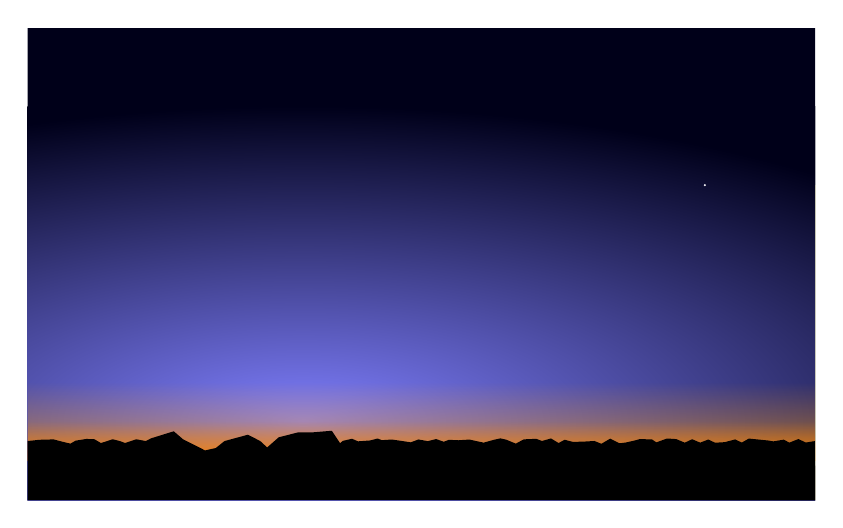
\begin{tikzpicture}
    
    \clip (-5,-3) rectangle (5,3);

    % the sky
    \fill[blue!10!black] (-6,1) rectangle (6,3);
    \fill[yellow] (-6,-3) rectangle (6,1);
    \fill[inner color=blue!50!,outer color=blue!10!black] (-12,-6) rectangle (9,2);

    % orange fadings
    \draw[draw=none] 
    [postaction={path fading=north,fill=orange!80!yellow,opacity=0.6}]
    (-7,-2.5) rectangle (7,-1.5);%
    \draw[draw=none] 
    [postaction={path fading=north,fill=orange,opacity=0.8}]
    (-7,-2.5) rectangle (7,-2);

    % the line of mountains
    \fill[black]
    decorate [decoration={random steps,segment length=3pt,amplitude=1pt}] %
    {(-5,-2.25) -- (-3.5,-2.25)}%
    decorate [decoration={random steps,segment length=5pt,amplitude=4pt}] %
    {-- (-2.5,-2.25) -- (-1,-2.25)}%
    decorate [decoration={random steps,segment length=3pt,amplitude=1pt}] %
    {-- (-1,-2.25) -- (5,-2.25)}%
    -- (5,-3) -- (-5,-3) -- (-5,-2.25);

    % a planet or a star
    \draw[color=white] (3.6,1) circle (0.005);
  \end{tikzpicture}  
\end{center}
\end{document}